
\begin{supplementary}

\section{Supporting Information}

\subsection{"dFBA" module}
We attempted to repurpose the C/C++ source code from the "dFBA" module for our intentions of developing a scalable module that is moreover accessible to all users. This process was derailed by a necessity to compile the “dfba\_utils.so” file in a UNIX operating system. A dynamic linked library (DLL) file was designed to replace the SO file; however, incompatibilities between C code in the library dependencies such as NVectors, SUNDIALS, and dlfcn and the C++ code the DLL file prevented this workaround. A further complication was that a few of these libraries, such as SUNDIALS, dynamically created the header files depending upon the user’s operating system systems; thus, a distinct DLL file would be required for each possible system architecture. The relative simple computational logic of the dFBA method compelled us to construct the simpler and ubiquitous dFBApy module without reference to this module. 

\subsection{Thermodynamic metabolism}
The kinetic dFBA algorithm was selected to define WCMpy metabolism as a convention of biochemistry, however, we also considered conducting metabolism through thermodynamics instead. This may foster an interesting contrast once both models are implemented within the WCMpy framework and are provided the same set of parameters, to definitively assess the suitability of each construct. The preliminary logic and calculations of this thermodynamic metabolic model are detailed in the following sections. 

\subsubsection{Membrane absorption}

\begin{figure}
    \centering
    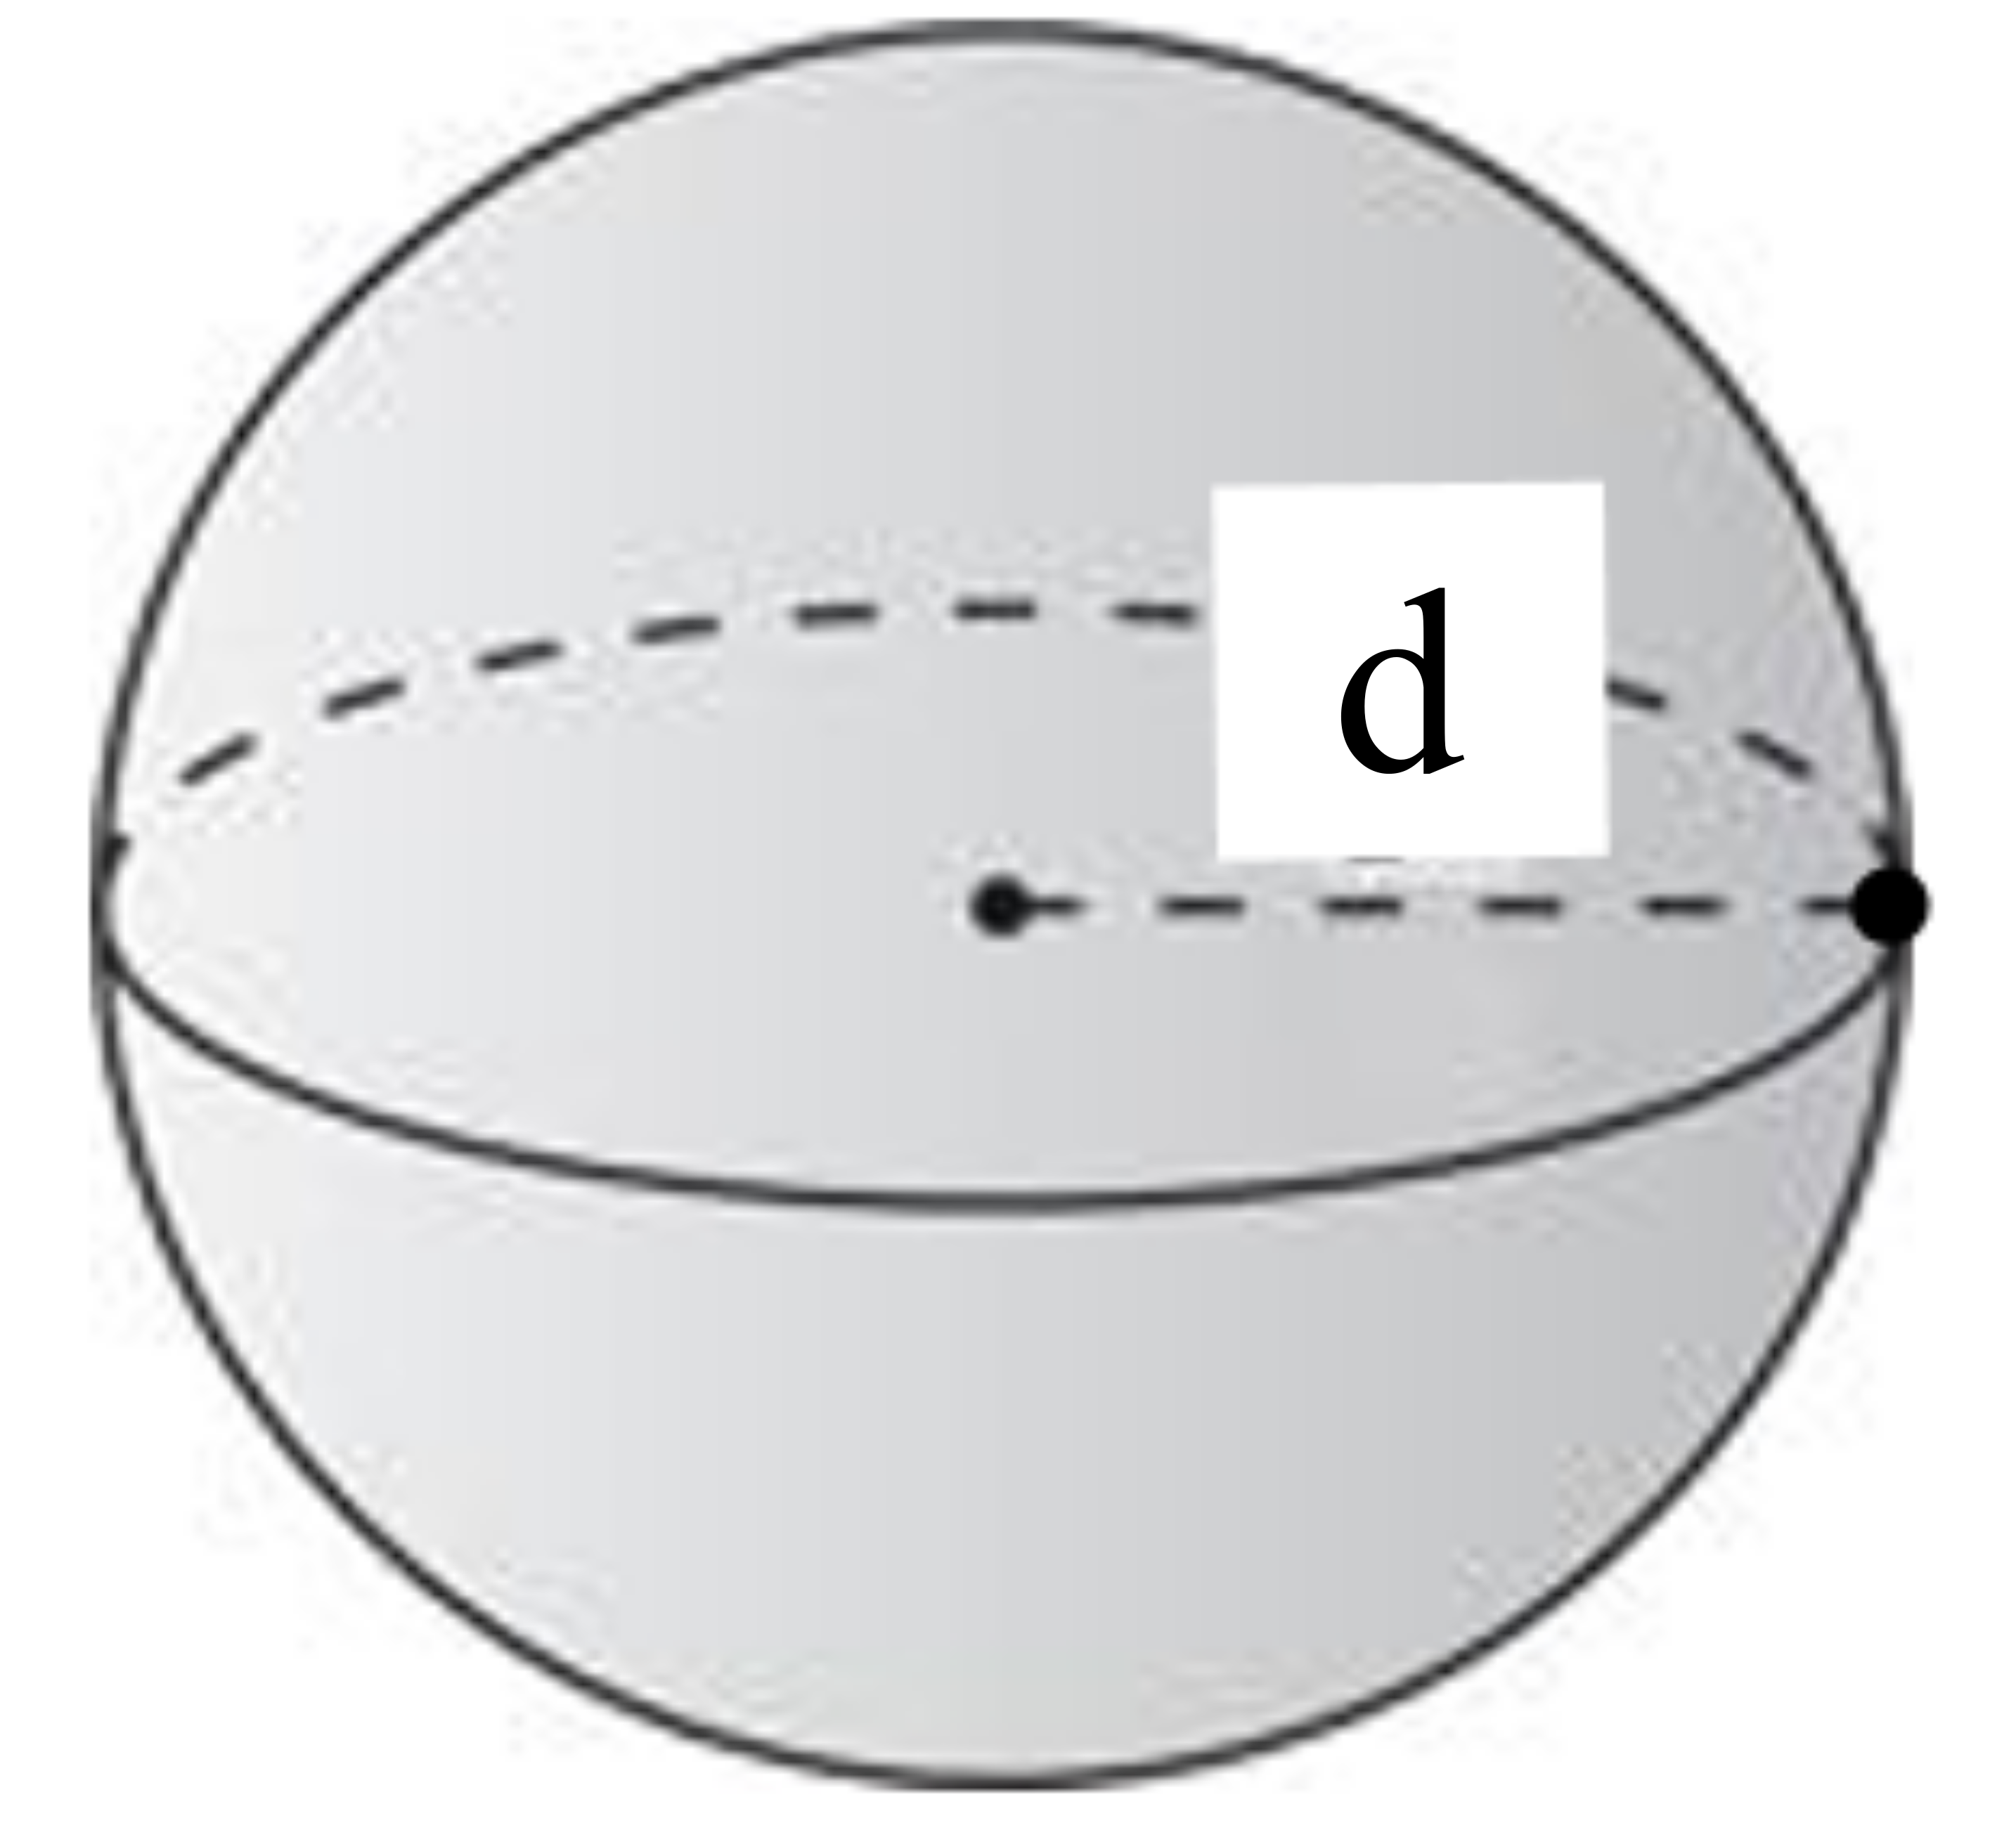
\includegraphics{images/WCMpy/diffusion_sphere.png}
    \caption{
        A sphere where the surface area represents the location of a chemical, which begins at the origin of the sphere, after a timestep and possessing the root-mean-squared velocity.
    }
    \label{diffusion_sphere}
\end{figure}

\begin{figure}
    \centering
    \begin{subfigure}[b]{0.45\textwidth}
        \centering
        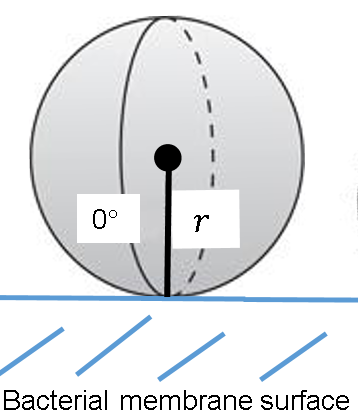
\includegraphics{images/WCMpy/maximal_far.png}
        \caption{
            The maximal distance. This radial distance defines the thickness of the volume shell around the bacterial membrane within which chemicals may potentially be absorbed.  
        }
    \end{subfigure}
    \hfill
    \begin{subfigure}[b]{0.45\textwidth}
        \centering
        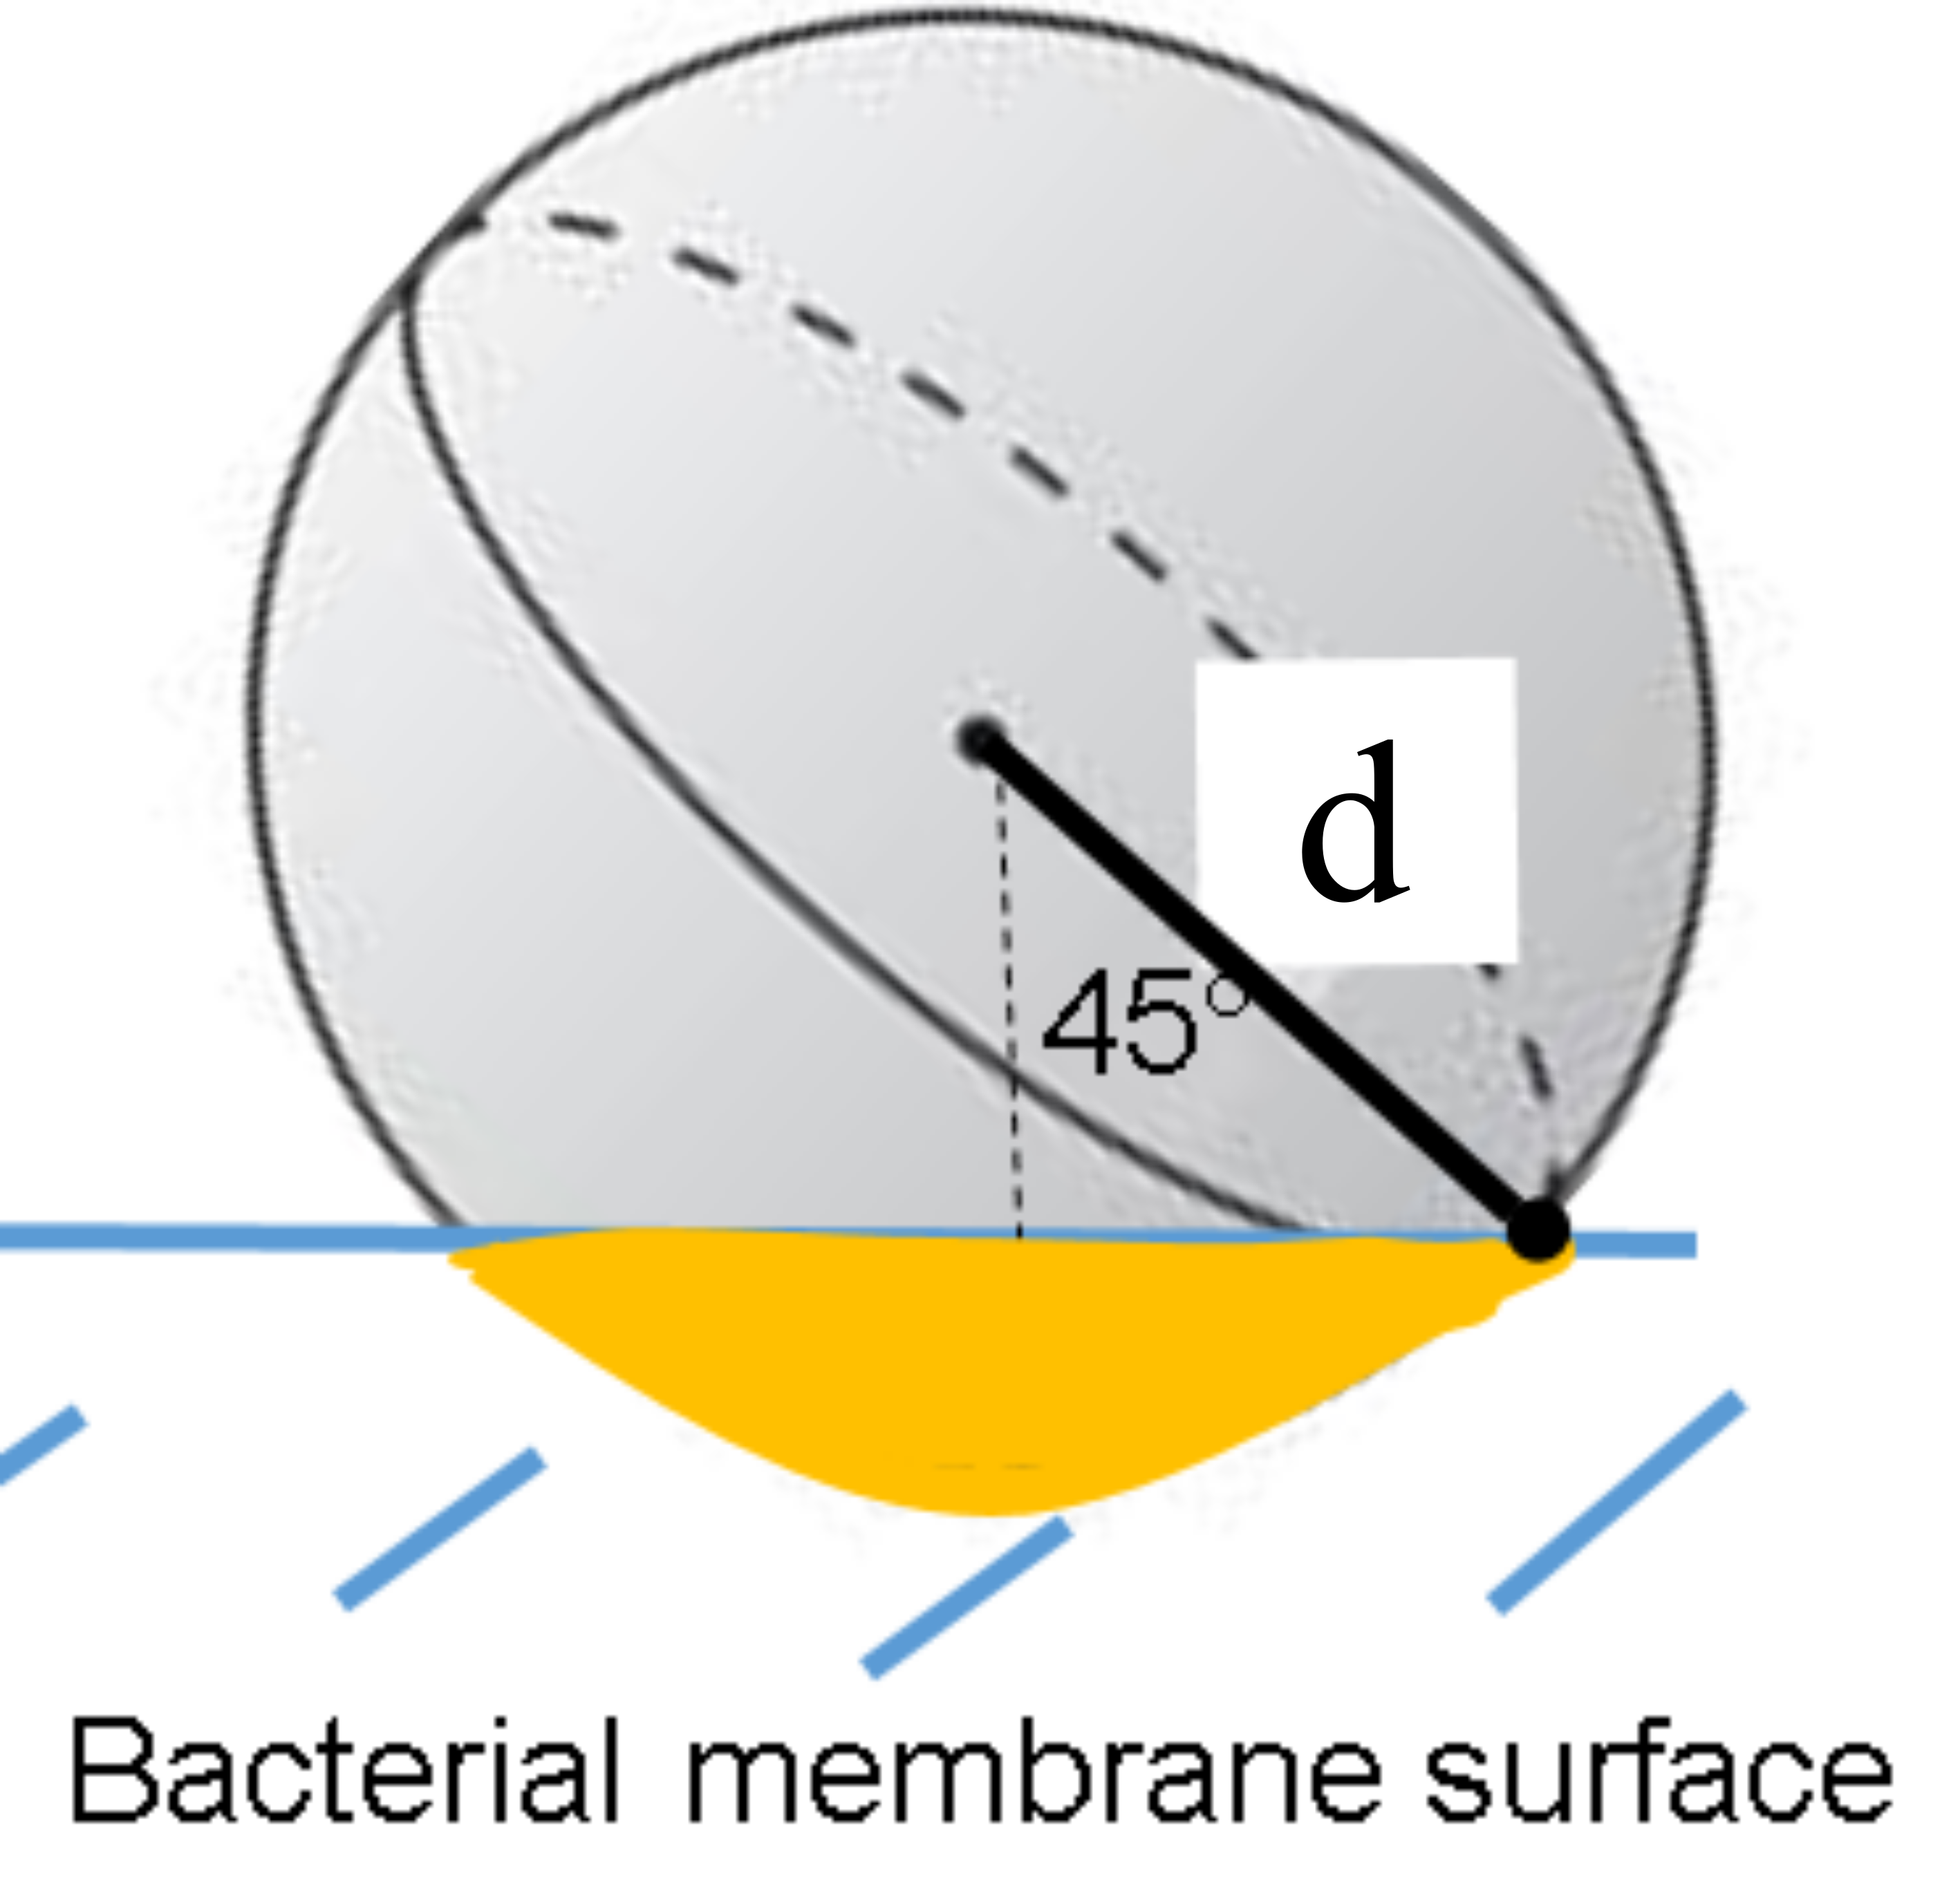
\includegraphics{images/WCMpy/average_far.png}
        \caption{
            The average distance. The proportion of surface areas of the orange region and the total sphere in \cref{collision_probability} represents the probability of that the average chemical within the volume shell around bacterial membrane collides with the membrane in the timestep.
        }
    \end{subfigure}
    \caption{
          Distances from the bacterial membrane a chemical can exist in the extracellular solution and still contact the membrane within the timestep.
    }
    \label{diffusion_distances}
\end{figure}

Cellular absorption is determined by the cellular dimensions, which are calculated with each timestep. The bacterial shape is assumed to be spherical, which facilitates calculations of the cellular volume and surface area as a function of cellular mass $m$ with each timestep, via a constant density, where $\frac{dm}{dt}=m_{absorption}-m_{excretion}$. The quantity of absorbed chemicals is calculated as a fraction of the chemicals that exist within a distance $d$ from the bacterial membrane,
\begin{equation}
    d=\overset{\rightharpoonup}{V}_{rms}*\Delta t~,
\end{equation} 
where a chemical, that possesses the root-mean-squared velocity of the average extracellular chemical, could feasibly interact with the bacterial membrane in a timestep $\Delta t$. The root-mean-squared velocity is expressed
\begin{equation}
    \overset{\rightharpoonup}{V}_{rms}=\sqrt{\frac{3*k_B*T}{m_{ave}}}
\end{equation} 		
where $k_B$ is the Boltzmann constant; $T$ is the extracellular temperature in kelvins; and $m_{ave}$ is the average mass of the extracellular chemicals. This $d$ distance is conceptually depicted as the radius of a sphere in Figure \ref{diffusion_sphere}, where the chemical at the start of the timestep resides at the spherical center and at the end of the timestep resides on the surface of the sphere, a $d$ distance from its origin. The volumetric shell of $d$ thickness around the bacterial membrane wherein chemicals can potentially be collide with the membrane and be absorbed is calculated
\begin{equation} \label{shell_volume}
    V_{shell}=\frac{4\pi}{3}*((d+r_{cell})^3-r_{cell}^3)
\end{equation}
where $r_{cell}$ is the cellular radius at the start of the $\Delta t$ timestep. The product of $V_{shell}$ and the extracellular chemical concentration $C_i$ of chemical $i$ 
\begin{equation} \label{shell_quantity}
    n_{shell,i}=C_i*V_{shell}
\end{equation}
yields the $n_{shell,i}$ quantity of chemical $i$ that resides in the $V_{shell}$ and may therefore be potentially absorbed. The proportion $P$ of $n_{shell,i}$ that will contact the membrane within $\Delta t$ is calculated as the proportion of surface area for possible locations that strike the membrane surface versus all possible locations for the average extracellular chemical after the $\Delta t$ 
\begin{equation} \label{collision_probability}
    P = \frac{SA_{membrane~collisions}}{SA_{sphere~of~possibilities}} = \frac{
    2*\pi*r_{distance~traveled}*(r_{distance~traveled}*cos(contact_angle))
    }{
    4*\pi*r_{distance~traveled}^2
    } = \frac{(cos(45\degree))}{2} = 14.6\%
\end{equation}
which is depicted in Figure \ref{diffusion_distances}. The contact angle of $45\degree$, between the extracellular chemical and the bacterial membrane, is the average between $90\degree$ for the infinitesimally close chemical to the membrane surface and $0\degree$ for the farthest possibly contacting chemical in Figure \ref{diffusion_distances}a. The $P$ value in \cref{collision_probability} is importantly an independent constant, while $n_{shell,i}$ scales proportionally with the $r$, $\overset{\rightharpoonup}{V}_{rms}$, and $T$. 

The fraction of these incident chemicals that are absorbed is approximated by its metabolic need $E$. This model estimates the $E_i$ of chemical $i$ as the deviation of the current thermodynamic displacement $\Pi_{R=1}^x (\frac{Q_R}{K_{eq, R}})$ -- for the $x$ number of $R$ reactions where a chemical $i$ is a reactant  -- from an optimum thermodynamic displacement that is calculated
\begin{equation}
    \left(\frac{Q}{K_{eq}}\right)_{optimum,i}=e^{\dfrac{\eta*n_{e^-}* F * E_{potential}}{R*T_{incubation}}}
\end{equation}
where $\eta$ is the total quantity of reactions in the bacterial membrane; $n_{e^-}$ is the average electron exchange of the membrane reactions where chemical $i$ is a reactant; $F$ is Faraday’s constant of electrical charge; $E_{potential}$ is the electrical potential of the bacterial membrane; $R$ is the gas constant; and $T_{incubation}$ is the incubation temperature of the simulated organism, which we presume to be indicative of the optimal thermodynamic displacement for the organism's biochemistry. The metabolic need
\begin{equation} \label{metabolic_need}
    E_i= \begin{cases}
            0, ~~\text{if} \left(\frac{Q}{K_{eq}}\right)_{optimum,i}<\Pi_{R=1}^x \left(\frac{Q_R}{K_{eq, R}}\right) \\
            \left(\frac{Q}{K_{eq}}\right)_{optimum,i}-\Pi_{R=1}^x \left(\frac{Q_R}{K_{eq, R}}\right), ~~\text{else}
        \end{cases} 
\end{equation}
is limited $E_i\ge0$ to prevent the jettison of chemicals which are in thermodynamic excess in the cytoplasm. The quantity of chemical $i$ that is absorbed in a timestep, in this model, 
\begin{equation}
    n_{absorbed,i}=E_i*n_i*P*B_i~,
\end{equation}
is the product of its metabolic need from \cref{metabolic_need}, its quantity in the volume shell from \cref{shell_volume,shell_quantity}, the probability of it striking the membrane \cref{collision_probability}, and finally the absorption hindrances $B_i$ that abstractly represent transport protein passage or other phenomena. The contribution to cellular mass growth from this absorption is calculated
\begin{equation} \label{mass_change}
    \frac{dm}{dt}=\sum_{i=1}^b(n_{absorbed,i}*MW_i)~.
\end{equation}
for all of the $b$ chemicals. The net change in cellular mass sums $\frac{dm}{dt}$ from \cref{mass_change} with the mass of ejected waste molecules from metabolic operation, which transpires changes in cellular volume and radius
\begin{equation}
    r_{cell}=\left(\frac{3*V_{cell}}{4*\pi}\right)^{\dfrac{1}{3}}    
\end{equation}
and subsequently the geometric calculations with each timestep. 


\subsubsection{Chemical reactions}

Metabolic reactions are partitioned between the cytoplasm (c), the membrane (m), and the extracellular environment (e). The maximal possible quantity of chemical reactions that can proceed in the forward or backward directions is calculated 
\begin{equation}
    R_{max}=\left|\frac{C_i}{s}\right| 
\end{equation}
where $C_i$ is the concentration of chemical $i$ and $s$ is the stoichiometry of the chemical $i$ in reaction $R$. The maximal $R_{max}$ reaction progressions in a $\Delta t$ is attenuated by a scalar $\zeta$ 
\begin{equation}
    R_{actual}=R_{max}*\zeta
\end{equation}
that represents unreactive collisions and diffusion limitations \cite{Feynman1963ChapterDiffusion}. The $R_{actual}$ is further limited by the quantity of enzymes that can catalyze the reaction \textit{e}
\begin{equation}
    R_{actual} = \begin{cases}
            R_{actual},~~if~R_{actual}<e \\
            e,~~else
            \end{cases}~.
\end{equation}
The concentration change $C_i$ -- in each separate compartment -- over the timestep for chemical $i$is calculated
\begin{equation}
    \frac{dC_i}{dt}=R_{actual}*s
\end{equation}
by the product of the quantity of reaction progressions by the respective stoichiometry of the chemical in the reaction. The new $C_i$ is crucially used in \cref{metabolic_need} to determine the metabolic need of the chemical in the system. 

Reaction direction is determined by the relative equality of $Q$ and $K_{eq}$
\begin{equation}
    NF = K_{eq}-Q~,        
\end{equation}
where $NF$ is the number of necessary forward reaction progressions and $-NF$ denotes backward reaction progressions. 

\end{supplementary}